\subsubsection{Map}
Loading a map enables viewing of geographic measurements made with a spectrogram and a GPS. Maps can be loaded from online API requiring an internet connection or loaded from a \textit{.pmtiles}-file for offline use. Compatible APIs and files are offered by several sources, the software \textit{QGis} offers support for exporting \textit{.pmtiles} from other formats using plugins.

\paragraph{Disclaimer} LuRaCs does not provide or distribute any map data. Users are responsible for ensuring that such data or tile services they use with LuRaCs are obtained and used in accordance with the applicable licenses, terms, and usage restrictions.

The map is rendered using Qt's web engine, making it a powerful but resource demanding tool. Using offline maps can require a lot of system memory since the server needs to cache tiles for a smooth view. It is therefore recommended to use a system with enough memory when this option is applied. However, both the map and datapoints are rendered using GPU acceleration with WebGL, allowing for 10 000s of points to be displayed without excessive stress on the system. For reference, a Raspberry Pi 5 with 8 GB of RAM can render a 1.4 GB map file without any stutter, total memory usage was approximately 2 GB.

\begin{figure}[H]
    \centering
    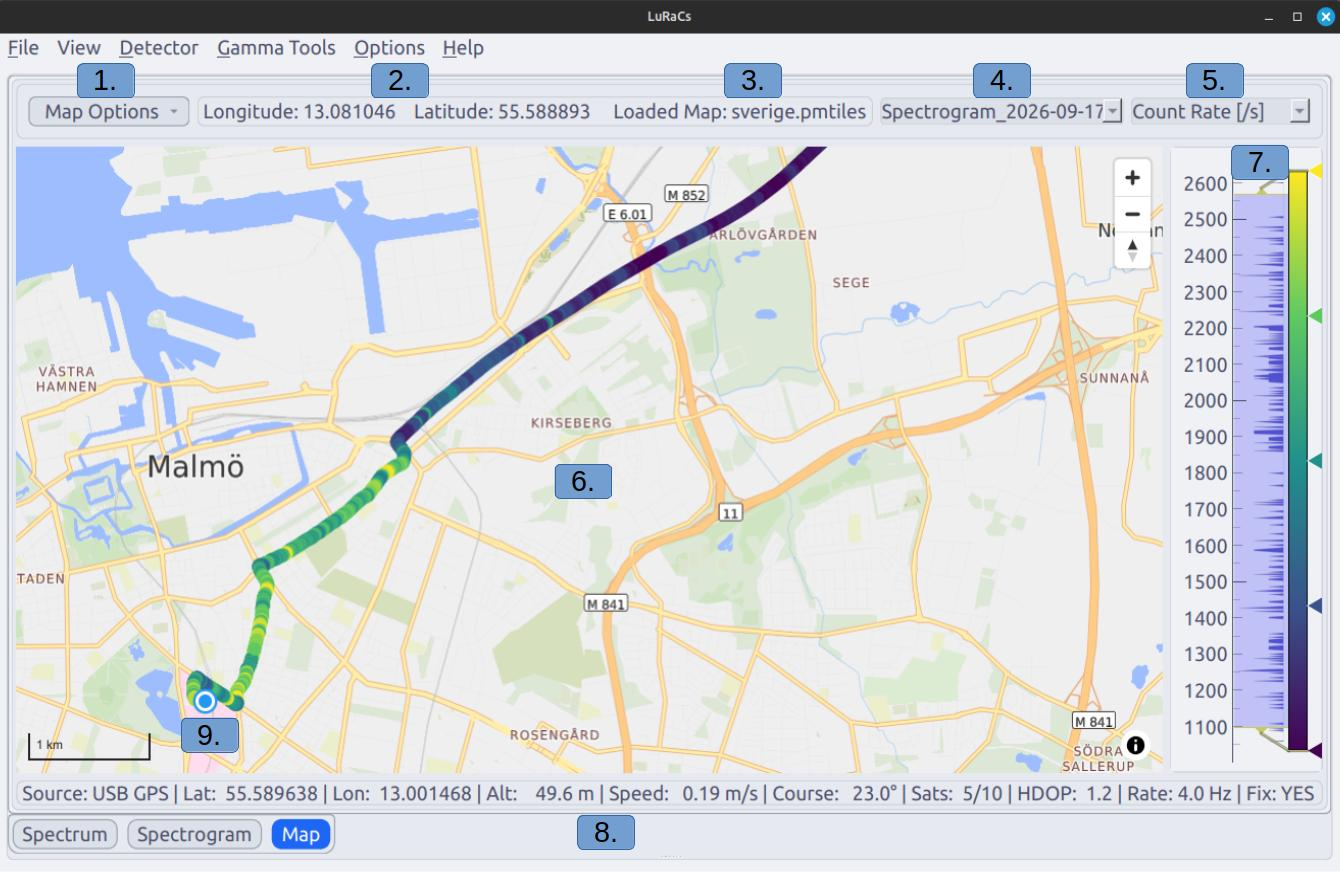
\includegraphics[width = .9\linewidth]{images/interface/map_view.jpg}
    \caption{Map with a loaded track and a connected GPS.}
    \label{fig:map_view}
    \begin{flushleft}
        \begin{enumerate}
            \item Options menu for loading maps, importing and exporting simple tracks.
            \item Longitude and Latitude for the position of the cursor.
            \item Name of the loaded map.
            \item List of loaded spectrograms. If the selected spectrogram does not contain any geolocation data, no measurement points are displayed.
            \item Selector for what data is shown: total count rate, dose rate or count rate inside a loaded ROI.
            \item Main map view.
            \item Selector for color gradient, used for the track points and a histogram over the measured values. The color map can be changed by clicking Mouse-2 on the gradient bar.
            \item Live data from the GPS.
            \item Current GPS position, always displayed as a white and blue circle.
        \end{enumerate}
    \end{flushleft}
\end{figure}

\paragraph{Load a map} is done from \texttt{Map Options -> Load Online/Offline Map}. An offline map takes the form of a \textit{.pmltiles} file. By choosing this option prompts the selection of such a file. Choosing to load an online map prompts the user to enter a URL, to a tile serving API, possibly including an API key. The checkbox allows for saving the most recently used URL. If a personal API key is used, be aware that URLs are saved unencrypted.